\documentclass[11pt]{article}
\usepackage[margin=1in]{geometry}
\usepackage{amsmath,amssymb,booktabs,graphicx}
\usepackage[round]{natbib}
\usepackage[hidelinks]{hyperref}
\newcommand{\CMAT}{CMAT}
\newcommand{\pending}[1]{\textbf{[TO COMPLETE: #1]}}
\title{Discovering Stable Attendance Regimes in University Mathematics Support: An Ordered Fusion Analysis}
\author{Author information withheld in working draft}
\date{Working draft --- October 2026}
\begin{document}
\maketitle

\begin{abstract}
Studies of university mathematics learning support typically distinguish service users from non-users, although recorded visit frequency is an ordered exposure whose empirical resolution is rarely examined directly. We develop an ordered fused-lasso framework for identifying contiguous visit-frequency regimes associated with final mathematics-course performance, without selecting attendance thresholds on the basis of favourable pairwise significance tests. Our setting is the first eligible attempt at a university mathematics course among students exposed to a support-centre attendance programme, building on a previously documented frequency analysis. We consider a binary pass indicator and instructor--period-standardised final performance with explicit adjustment for instructor--period and degree programme. We propose penalising only differences between adjacent visit-frequency coefficients, selecting the penalty via cluster-respecting conditional cross-validation, assessing boundary stability through whole-cluster bootstrap, and evaluating discovered boundaries on reserved instructor--period clusters with unpenalised, cluster-robust Wald contrasts. For standardised grades, the selected partition was $[0]|[1+]$ and the $0|1$ boundary appeared in all 100 cluster-bootstrap replicates. Validation in 1,952 reserved observations estimated an adjusted 0.264-standard-deviation difference (95\% CI 0.150--0.377). For PASS, the conservative cross-validation heuristic fused all frequencies, although the $0|1$ boundary appeared in 37\% of bootstrap replicates and competing discovery-fit criteria favoured additional separation. The proposed framework distinguishes stable descriptive regimes from equivalence, causal dose-response thresholds and algorithmic artefacts.
\end{abstract}

\noindent\textbf{Keywords:} mathematics support; attendance frequency; ordered categorical predictors; fused lasso; total variation; clustered validation; post-selection inference.

\section{Introduction}
University mathematics-support programmes are usually evaluated using observed uptake and later academic outcomes, despite the substantial differences between a first visit and repeated attendance \citep{matthews2013,lawson2020,mullen2024}. Attendance is not randomly assigned. Students may attend because they experience mathematical difficulty, seek opportunities to consolidate knowledge, respond to an institutional participation incentive, or combine these motivations. Consequently, associations between attendance and final performance should not be described as treatment effects.

Existing observational evaluations often contrast any use with none \citep{macanbhaird2009,rickard2018,jacob2019}; identification-oriented work highlights how this association may differ from causal effects under self-selection \citep{paloyo2016,pugatch2018,buchele2024}. A separate question concerns repeated engagement and whether each recorded number of visits warrants a separate adjusted outcome coefficient. A conventional eight-level factor permits all means to differ, but high-frequency levels are sparse, and 28 pairwise contrasts can be difficult to interpret. Ordered fusion regularises successive coefficient differences rather than assuming a linear dose response; it is closely related to the fused-lasso and generalised-lasso literature \citep{tibshirani2005fused,tibshirani2011generalized}. Conversely, pooling levels a priori may conceal substantively meaningful variation.

The preceding CMAT frequency study considered the ordered grid $0,1,2,3,4,5,6,7+$ and documented a strong non-user/user outcome separation, while comparisons among positive frequencies were substantially less decisive after multiplicity control. Its earlier outcome-blind overlap audit had favoured a pooled $6+$ upper tail, whereas its later eight-level reporting grid was exploratory. Those observations motivate this study but do not predetermine the location or number of boundaries. We ask whether a data-adaptive but explicitly validated method can reveal stable \emph{contiguous attendance regimes}, thereby replacing post-hoc inspection of pairwise $p$-values with a transparent ordered estimation problem.

The study is deliberately observational. A boundary that recurs in administrative data is not a causal tipping point, and fusion does not prove equality of adjacent population means. During at least part of the historical observation period, an institutional participation-credit programme could be satisfied through three visits, so the $2|3$ and $3|4$ boundaries have potential institutional meaning but are not assigned privileged inferential status.

\section{Setting, cohort and outcomes}
The starting cohort is the first eligible attempt at Matem\'aticas Universitarias during a period with CMAT coverage, with attendance measured within the same academic period, as defined by the preceding study. Students are compared in instructor--period grading contexts. Let $K_i\in\{0,1,2,3,4,5,6,7+\}$ denote visit frequency, $C_i$ instructor--period and $D_i$ degree programme.

Our binary outcome is $PASS_i=1$ for an observed numeric final grade of at least $7.5$, and $0$ for a lower numeric grade or adverse administrative code BA, BV or RT, following the fixed inherited outcome contract. The continuous primary outcome, $Z_i$, uses the earlier specified adverse-outcome mapping and standardisation within instructor--period; numeric complete-case $Z$ is a sensitivity. The binary and continuous outcomes answer different questions, since passing is a threshold event while $Z$ retains within-course performance differences.

\pending{Verify the current frozen cohort and the number of students and independent classroom/instructor clusters in each discovery and validation subset; include a disclosure-safe flow diagram.} The full $7+$ grid is the primary discovery specification; pooling $6+$ remains an a priori support sensitivity rather than a redefinition chosen after inspecting outcomes.

\section{Methods}
\subsection{Ordered fused-lasso model}
For either outcome $Y_i$, we estimate an additive model with unpenalised instructor--period and degree nuisance effects. Let $\gamma_k$ represent the adjusted level associated with visit frequency $k$, under an explicit location constraint. Our fusion-only penalty differs from the original formulation that can also penalise coefficient magnitudes; the target here is local constancy, not eliminating the attendance predictor. Our penalised criterion is
\begin{equation}
\min_{\boldsymbol\gamma,\boldsymbol\alpha,\boldsymbol\delta}
\frac{1}{2n}\sum_{i=1}^{n}
\left(Y_i-\gamma_{K_i}-\alpha_{C_i}-\delta_{D_i}\right)^2
+\lambda\sum_{k=1}^{7}|\gamma_k-\gamma_{k-1}|.
\label{eq:fusion}
\end{equation}
Here $k=7$ denotes the pooled $7+$ level rather than an exact seventh visit. The total-variation penalty acts \emph{only} on adjacent frequency coefficients; contextual and degree effects are not penalised. Writing $d_k=\gamma_k-\gamma_{k-1}$ transforms the problem into a lasso on seven cumulative-step regressors after partialling out nuisance effects. At $\lambda=0$ the model is the unrestricted fixed-effect OLS/LPM; for sufficiently large $\lambda$, all adjacent contrasts are zero and a single frequency regime remains.

A nonzero estimated $d_k$ defines a boundary $k-1|k$. Zero estimated differences generate contiguous blocks, but fused-lasso solutions do not guarantee a nested agglomerative dendrogram as $\lambda$ varies. Eight ordered categories admit $2^7=128$ possible contiguous partitions; a later exhaustive-partition exercise may benchmark the penalised path without redefining this study as a search for a predetermined four-block pattern.

\subsection{Penalty selection and clustered prediction}
We reserve entire instructor--period clusters as an untouched validation sample. Within the discovery clusters, the penalty is selected using grouped cross-validation. Since a previously unseen instructor--period cannot have an intercept estimated in the training data, the criterion is a \emph{within-held-out-context} prediction loss: for each held-out classroom, predicted attendance and degree contributions are subtracted from the observed outcome and the remaining classroom-specific mean is removed. The resulting mean squared error measures prediction of within-context differences, not a promise to predict absolute grades for an unseen instructor.

We compare a grid containing $\lambda=0$, intermediate penalties and a value sufficient for complete fusion. A one-standard-error-type \emph{heuristic} favours the most parsimonious penalty whose cross-validation score is near the minimum. Correlated folds do not support a naive inferential interpretation of this heuristic standard error. The penalty, split seed, weighting, regularisation scaling and minimisation settings are recorded in a reproducibility manifest.

\subsection{Bootstrap stability}
To determine whether a selected cut is stable rather than a feature of one sample, we resample whole discovery instructor--period clusters, repeat penalty tuning and re-estimate the partition. For each of seven possible boundaries we report the fraction of successful bootstrap fits that retained the boundary, together with failures and selected block-count frequencies. These are descriptive \emph{selection frequencies}, not posterior probabilities or $p$-values. Although motivated by the broader stability-selection literature \citep{meinshausen2010stability}, this classroom bootstrap should not be claimed to inherit its formal error-rate guarantees. A planned instructor-level resampling sensitivity addresses dependence spanning multiple periods.

\subsection{Independent post-selection inference}
Penalised coefficients are deliberately shrunken and ordinary Wald tests on them are not justified. Valid inference after model selection is a distinct statistical problem \citep{lee2016postselection}; we use reserved-cluster validation rather than asserting that a same-sample unpenalised refit resolves selection uncertainty. Moreover, an unpenalised refit on the same observations used to select boundaries would not remove post-selection bias. We therefore freeze the discovery partition and perform the unpenalised block-factor regression using only the reserved validation clusters. For a selected adjacent-block contrast $a^\top\theta$, the test statistic is
\begin{equation}
Z=\frac{a^\top\widehat{\theta}}{\sqrt{a^\top\widehat V_{\mathrm{CR}}a}},
\end{equation}
where $\widehat V_{\mathrm{CR}}$ allows arbitrary within-instructor--period error correlation under standard cluster-asymptotic conditions. Separate predeclared families of selected adjacent contrasts for $Z$ and PASS are adjusted using Holm's procedure; binary differences are reported in percentage points. The number and support of validation clusters are reported alongside all intervals. An unidentifiable boundary is marked untestable, never silently merged or declared non-significant.

This sample-splitting design sacrifices precision but avoids using a selected contrast's own validation outcomes to choose it. It does not remove confounding associated with voluntary attendance, establish within-block equivalence, or confer causal meaning on an observed regime boundary.

\subsection{Sensitivity and reporting}
We compare the eight-level and historically supported pooled-$6+$ grids, assess numeric-complete-case outcomes, record sparse-tail overlap, and contrast the selected partition with unrestricted eight-level and simple zero-versus-positive descriptive benchmarks. We report both outcomes independently, without presuming they yield identical partitions. \pending{If repeated split/sample-stability designs or instructor-level clustering are added, document them before their results are inspected.}

\section{Results}

\subsection{Cohort and estimation sample}
The cohort comprised 6,627 first eligible mathematics-course attempts in 190 instructor--period clusters. The cluster-level split reserved 1,952 students from 57 clusters for validation and allocated 4,675 students from 133 clusters to discovery. In the eight-category visit grid, 5,393 students reported no visits, while the respective counts for exact one through six visits and seven or more were 517, 245, 170, 96, 55, 50 and 101. Both outcomes and both upper-tail representations completed 100 out of 100 cluster-bootstrap fits, with no recorded failures.

\subsection{Selected attendance regimes}
For instructor--period-standardised grades, the discovery-sample ordered fused lasso selected two blocks: $[0]$ and $[1,2,3,4,5,6,7+]$, using $\lambda=0.028091$. The same division emerged when exact six visits were pooled with the upper tail as $6+$. Among all 128 contiguous eight-category partitions, this two-block solution also had the most favourable discovery-sample relative BIC.

For PASS, the conservative one-standard-error-style cross-validation heuristic selected an all-fused single block at $\lambda=0.024082$. Importantly, the minimum grouped-CV loss occurred at $\lambda=0.000360$, with MSE 0.168915 versus 0.173192 for the selected all-fused model. The latter difference was permitted by the four-fold estimated tolerance, which is a parsimony heuristic rather than an inferential standard error. The discovery-only Gaussian-working-model BIC ranked the all-fused solution last of 128; its best-ranked alternative had cuts $0|1$ and $3|4$, followed by $0|1$ alone (relative BIC difference approximately 1.53). Neither ranking is a held-out hypothesis test, and changing the selection rule after observing these results would require explicitly labelled sensitivity analysis.

\subsection{Bootstrap boundary stability}
Table~\ref{tab:selection} reports selection frequencies from 100 successful whole-classroom bootstrap replicates, each repeating lambda selection. For standardised grades, the initial $0|1$ boundary was selected in every replicate, while no other positive-frequency boundary exceeded 10\%. For PASS, the same initial boundary appeared in only 37\% of replicates. Frequencies of selected cuts are neither $p$-values nor measures of equivalence within fused blocks.

\begin{table}[ht]
\centering
\caption{Frequency of selecting each primary-grid visit boundary in 100 cluster-bootstrap replicates.}
\label{tab:selection}
\begin{tabular}{lrr}
\toprule
Visit boundary & Standardised grade (\%) & PASS (\%)\\
\midrule
$0|1$ & 100 & 37\\
$1|2$ & 10 & 2\\
$2|3$ & 0 & 0\\
$3|4$ & 1 & 1\\
$4|5$ & 0 & 0\\
$5|6$ & 0 & 0\\
$6|7+$ & 0 & 0\\
\bottomrule
\end{tabular}
\end{table}

\IfFileExists{../../results/paper221/figures/7plus_z_grade_primary_boundary_stability.pdf}{
\begin{figure}[ht]
\centering
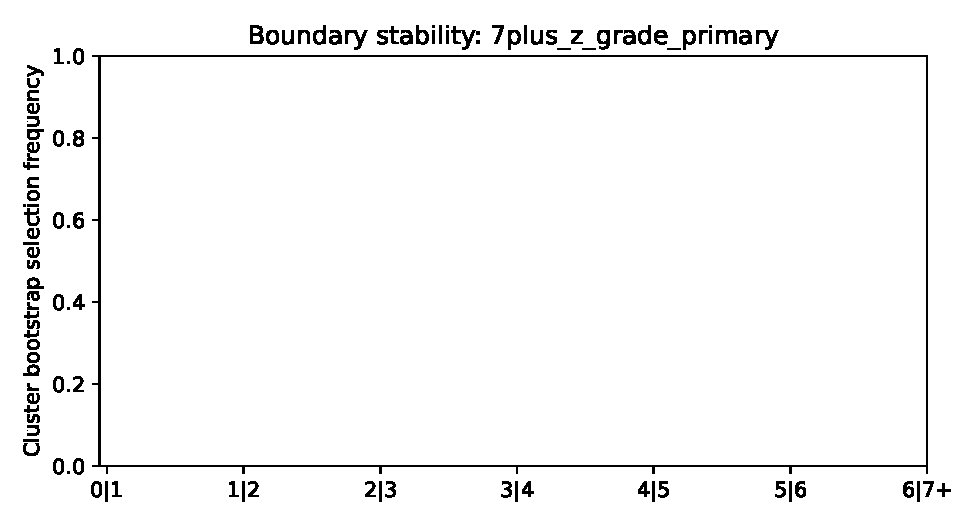
\includegraphics[width=.8\linewidth]{../../results/paper221/figures/7plus_z_grade_primary_boundary_stability.pdf}
\caption{Selection frequency of each adjacent cut for standardised grades. The penalisation is reselected in each discovery-classroom bootstrap sample.}
\end{figure}
}{}

\IfFileExists{../../results/paper221/figures/7plus_pass_boundary_stability.pdf}{
\begin{figure}[ht]
\centering
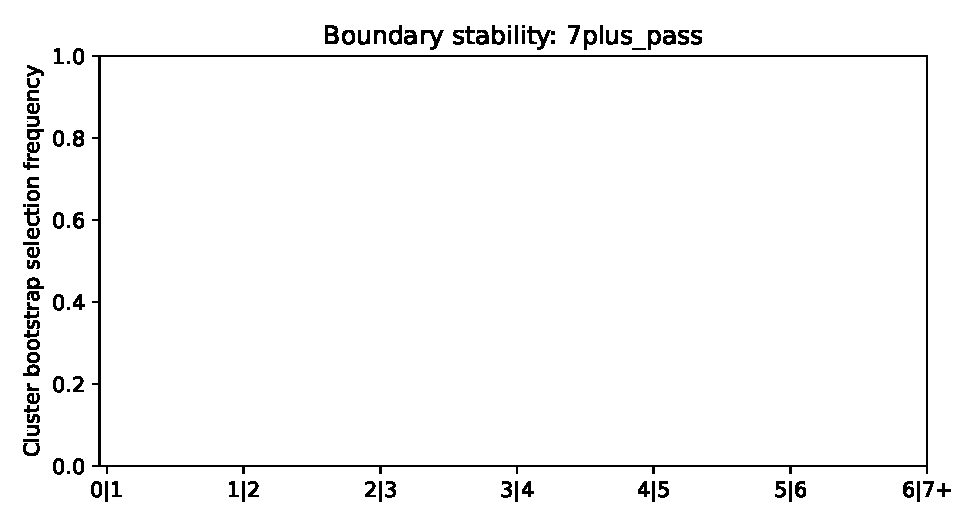
\includegraphics[width=.8\linewidth]{../../results/paper221/figures/7plus_pass_boundary_stability.pdf}
\caption{Corresponding bootstrap selection frequency for the PASS outcome; an all-fused model is a penalised representation, not an equivalence test.}
\end{figure}
}{}

\subsection{Reserved-cluster validation}
Refitting the two selected Z blocks without penalisation in the 57 reserved instructor--period clusters gave an adjusted difference of 0.2636 standard deviations between students with at least one visit and students with none (cluster-robust standard error 0.0580, nominal 95\% CI 0.150--0.377, Wald and Holm-adjusted $p=5.44\times10^{-6}$). Among 1,952 validation observations, 1,585 had zero visits and 367 had positive visits; 52 clusters contained both blocks. PASS selected no boundary and therefore has no corresponding selected-boundary Wald test. Its absence is not evidence of a zero effect.

The new fusion algorithm did not use validation outcomes for its tuning or bootstrap. Nevertheless, these observations belong to the wider cohort already examined in Paper 2.1, so this analysis offers \emph{internal algorithmic validation}, not a prospectively untouched or externally replicated confirmatory sample.

\subsection{Tail-pooling and pending sensitivities}
The pooled-$6+$ analysis reproduced the same grade and PASS partitions, with the $0|1$ boundary selected in 100\% and 37\% of bootstrap replicates, respectively. Numeric complete-case Z, instructor-level dependence, repeated grouped folds and a minimum-CV-loss penalty-selection sensitivity remain to be evaluated; the published estimates should not be described as robust to these unperformed analyses.


\section{Discussion}
The central scientific object is not a causal marginal return to each additional visit, but the empirical \emph{resolution} supported by an ordered exposure under contextual adjustment. Fusion can express a potentially broad first-use separation while allowing evidence-supported boundaries at repeated visits, yet may also correctly return few or no extra regimes. Since equal fitted coefficients arise from a penalty and a non-rejected difference does not establish equivalence, reported blocks are parsimonious representations rather than proven homogeneous populations.

Several limitations govern interpretation. Voluntary attendance and unmeasured mathematical preparation may confound all observed relations. Some upper-tail frequencies occur in few instructor--period clusters and can yield unstable boundaries. The administrative treatment of non-numeric outcomes affects the continuous outcome and must be audited against numeric complete cases. Held-out conditional scoring removes unseen classroom intercepts; its target differs from unconditional student-level predictive accuracy. Bootstrap selection proportions quantify algorithmic sensitivity to resampling but not inferential certainty regarding population thresholds. Finally, independent-cluster validation may have inadequate support for rare blocks, in which case abstaining from a significance claim is necessary.

The clear standardised-grade $0|1$ result agrees with the original zero-versus-positive attendance contrast in the prior paper, although the selected fusion of all positive levels does not imply within-block equivalence. For PASS, the all-fused result is highly sensitive to the parsimony heuristic: the minimum CV loss occurs at a substantially smaller penalty and the discovery-only BIC ranks the selected model last. Further tuning and dependence sensitivities are needed before a substantive PASS conclusion. Because the wider institutional cohort was already explored in Paper 2.1, this split is an internal validation of the new algorithm rather than an independently collected confirmatory study.

\section{Conclusion}
A one-dimensional ordered fused-lasso analysis selected a robust initial-use boundary for standardised grades, with 100\% classroom-bootstrap selection and a positive adjusted difference in reserved classroom clusters. For PASS, the selected regime count depends on a conservative tuning rule. These patterns describe attendance-associated outcomes, not causal returns to further visits.

\section*{Declarations}
\pending{Insert exact institutional data-use, ethics/approval language, funder declarations, author contributions, availability terms and verified submission requirements. No row-level administrative data will be released.}

\bibliographystyle{plainnat}
\bibliography{../references,methods_references}
\end{document}
